\subsection{Predicting log-volatility}
\label{sec:stochastic:volatility}

As a first numerical illustration we consider the problem of computing the predictor flow in the---now classical---stochastic volatility model 
\begin{equation} \label{eq:sto:vol:model}
	\begin{split}
		X_{n + 1} &= \varphi X_n + \sigma U_{n + 1}, \\
		Y_n &= \beta \exp \left( X_n / 2 \right) V_n,   
	\end{split}
	\quad n \in \nset, 
\end{equation}
proposed in \cite{hull:white:1987}, where $\{ U_n \}_{n \in \nsetpos}$ and $\{ V_n \}_{n \in \nset}$ are sequences of uncorrelated standard Gaussian noise. In this model, where only the process $\{ Y_n \}_{n \in \nset}$ is observable, $\beta$ is a constant scaling factor, $\varphi$ is the \emph{persistence}, and $\sigma$ is the \emph{volatility of the log-volatility}. In the case where $|\varphi| < 1$, the state process $\{ X_n \}_{n \in \nset}$ is stationary with a Gaussian invariant distribution having zero mean and variance $\tilde{\sigma}^2 \eqdef \sigma^2 / (1 - \varphi^2)$.  

It is easily checked that the model $\{ (X_n, Y_n) \}_{n \in \nset}$ defined by \eqref{eq:sto:vol:model} is indeed a state-space model in the notion of Example~\ref{example:state:space:model}, and in this case $\Xsp = \Ysp = \rset$, $\Xfd = \Yfd = \mathcal{B}(\rset)$, and  
\[
	\begin{split}
		\mk(x, A) &= \int_A \phi(x' ; \varphi x, \sigma^2) \, \rmd x', \\
		\pot(x, y) &= \phi(y ; 0, \beta^2 \me^x),  
	\end{split}
\]
where $(x, y) \in \rset^2$, $A \in \mathcal{B}(\rset)$, and $\phi(\cdot ; \mu, \varsigma^2)$ denotes the density of the Gaussian distribution with expectation $\mu \in \rset$ and standard deviation $\varsigma > 0$. Consequently, the flow of one-step log-volatility predictors satisfies the perturbed Feynman-Kac recursion \eqref{eq:pred:rec} with $\pot[y] = \ed(\cdot, y)$, $y \in \Ysp$, and may thus be approximated using SMC methods. 

We check that the model satisfies the simplified assumptions in Remark~\ref{rem:simplified:assumptions} for the scenario where $|\varphi| < 1$, implying stationary state and observation processes, the latter with marginal stationary distribution 
\begin{equation} \label{eq:stationary:marginal:observations}
	\mathcal{B}(\rset) \ni A \mapsto \iint \1_A(y) \phi(y ; 0, \beta^2 \me^x) \phi(x ; 0, \tilde{\sigma}^2) \, \rmd x \, \rmd y. 
\end{equation}
For this purpose, we first note that for all $y \in \rset$,
$$
	\| \pot[y] \|_\infty = \frac{1}{|y| \sqrt{2 \pi}} \me^{-1/2}, 
$$
i.e., for all $(x, y) \in \rset^2$, 
\begin{equation*}
	\frac{\pot[y](x)}{\| \pot[y] \|_\infty} \propto |y| \exp \left( - \frac{x}{2} - \frac{y^2 \me^{- x}}{2 \beta^2} \right), 
\end{equation*}
where the right hand side tends to zero as $|x| \rightarrow \infty$ for all $y \in \rset$. We thus conclude that Conditions~\eqref{item:condition-L-K} and \eqref{item:condition:local:doeblin:simplified} in Remark~\ref{rem:simplified:assumptions} hold true for any compact set $K \subset \rset$ with probability exceeding $2/3$ under \eqref{eq:stationary:marginal:observations}. In this case, every compact set $C \subset \rset$ is $1$-local Doeblin with respect to Lebesgue measure. In addition, since 
\begin{equation} \label{eq:finite:second:moment:obs:process}
	\E \left[Y_0^2 \right] = \beta^2 \int \me^x \phi(x ; 0, \tilde{\sigma}^2) \, \rmd x < \infty, 
\end{equation}
Condition~\eqref{item:mino-g-simple} is satisfied for all compact sets $D \subset \rset$. Moreover, for such compact sets $D$, \eqref{eq:finite:second:moment:obs:process} implies that $\mdr(D, 1)$ contains all initial distributions $\init$ with $\init(D) > 0$; in particular,  $\mdr(D, 1)$ contains the invariant Gaussian distribution of the state process, which we use as initial distribution in the predictor Feynman-Kac recursion. 

In this context, we aim at computing the sequence $\{ \pred[\chunk{y}{0}{n - 1}] \operatorname{id} \}_{n \in \nset}$ of predictor means; however, due to the nonlinearity of the emission density $\pot$, closed-form expressions are beyond reach, and we thus apply SMC for this purpose. In the scenario considered by us, $(\beta, \varphi, \sigma) = (.641, .975, .165)$, which are the parameter estimates obtained in \cite[Example~11.1.1.2]{cappe:moulines:ryden:2005} on the basis of British pound/US dollar daily log-returns from 1~October 1981 to 28~June 1985. In this setting, the following two numerical experiments were conducted.  

\subsubsection{Lag size influence}
\label{sec:lag:size:influence}

First, in order to assess the dependence of the bias \eqref{eq:def:bias} on the lag $\lag$, a record comprising $600$ observations were generated by simulation of the model under the parameters above. We re-emphasise that even though we here, for simplicity, consider the scenario of a perfectly specified model, this is not required in our assumptions in Section~\ref{sec:theoretical:results} (as long as the observation sequence is stationary). By inputting, $100$ times, these observations into Algorithm~\ref{alg:fixed-lag:SMC} and running the same with $\N = 4000$ particles, $100$ replicates of the particle predictor mean at time $600$ were produced and furnished with estimates of the asymptotic variance at the same time point. For each replicate, the asymptotic variance was estimated using all the lags $\lag \in \{2, 10, 12, 14, 16, 18, 20, 22, 50, 100, 200, 600\}$, where the last one, $\lag = 600$, corresponds to the CLE. Moreover, the reference value $1.63$ of the asymptotic variance, again at the time point $600$, was obtained by the brute-force approach consisting in generating as many as $1000$ replicates of the particle predictor mean, again with $\N = 4000$ particles, and simply multiplying the sample variance of these replicates by $\N$. The outcome is reported numerically and visually in Table~\ref{tab:lags:means:stds:stovol} and Figure~\ref{fig:boxplots:stovol}, respectively, where the different boxes in Figure~\ref{fig:boxplots:stovol} correspond to different lags. For each box, the reference value is indicated by a blue-colored asterisk $(\ast)$ and the average estimate of each box is indicated by a red ditto. From Figure~\ref{fig:boxplots:stovol} it is evident that the clear bias introduced by the smallest lags ($\lag \in \{2, 10, 12\}$) decreases rapidly as $\lag$ increases, and for $\lag = 20$ the bias is more or less eliminated. After this, increasing further $\lag$ leads, as we may expect from the particle path degeneracy, to significant increase of variance and no further improvement of the bias. On the contrary, the fact that the cardinality of the set $\{\enoch{\lagtime{n}{\lambda}}{n}{i} : i \in \intvect{1}{\N} \}$ decreases monotonously as $\lag$ increases, leading to constantly zero variance estimates for $n$ and $\lambda$ large enough, re-introduces bias also for large $\lag$. For the last replicate, the cardinalities of the sets $\{ \eve{n}{i} : i \in \intvect{1}{\N} \}$ and $\{\enoch{\lagtime{n}{20}}{n}{i} : i \in \intvect{1}{\N} \}$ were $8$ and $140$, respectively.  
\begin{figure}[H] 
    %\vspace{-25mm}
    \centering
    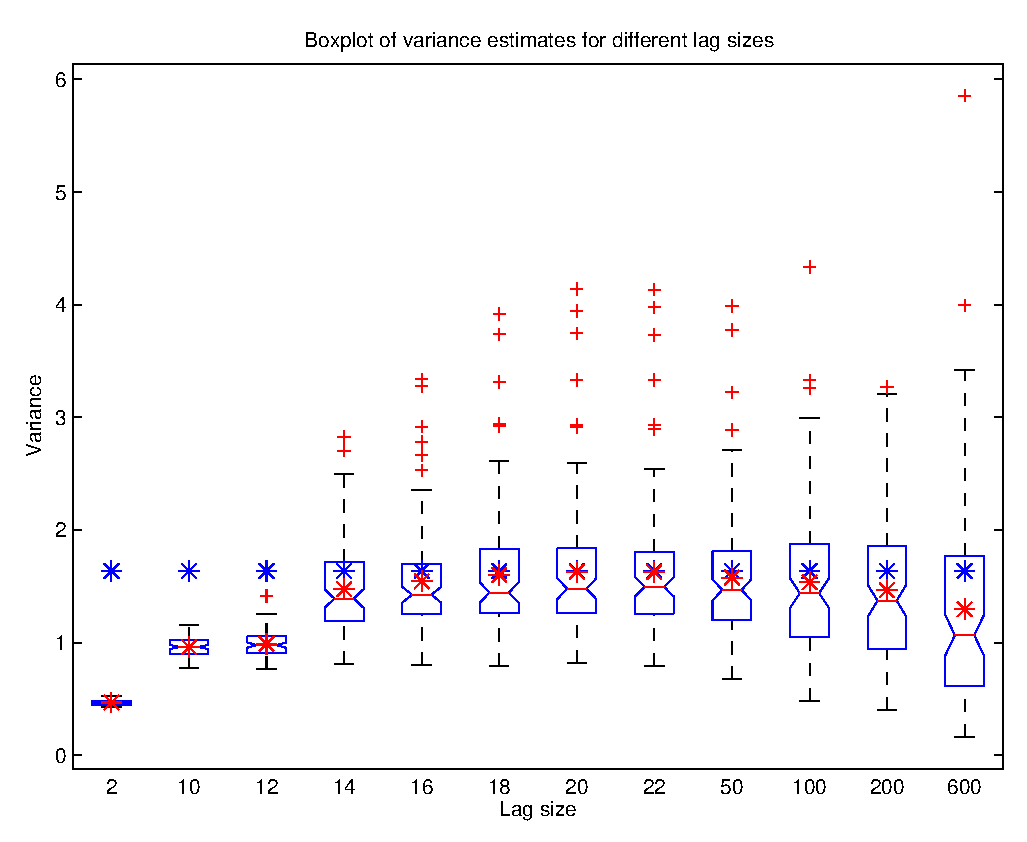
\includegraphics[width=0.8\textwidth]{boxplots_161211} % Data in fixed_lag_stovol_161211.mat
    %\vspace{-30mm}
    \caption{Estimated asymptotic variances of the particle predictor mean at time $600$ in the stochastic volatility model \eqref{eq:sto:vol:model}. The particle population size is $\N = 4,\!000$. The boxes are based on $100$ replicates of Algorithm~\ref{alg:fixed-lag:SMC} and correspond to the different lags $\lag \in \{2, 10, 12, 14, 16, 18, 20, 22, 50, 100, 200, 600\}$. The reference value $1.63$, which is indicated by blue-colored asterisks $(\ast)$, was obtained as the sample variance (scaled by the number of particles) of $1000$ independent replicates of the particle predictor mean at time $600$ (again, Algorithm~\ref{alg:fixed-lag:SMC} used $\N = 4000$ particles). Red-colored asterisks indicate average estimates.} \label{fig:boxplots:stovol}
\end{figure}

\begin{table}[H] \label{tab:lags:means:stds}
    \begin{center}
        \begin{tabular}{c|c|c} \toprule
            $\lambda$ & Mean & St. dev. \\ \midrule 
            $2$     & $.47$   & $.02$ \\
            $10$   & $.96$   & $.09$ \\ 
            $12$   & $.99$   & $.11$ \\
            $14$   & $1.47$& $.40$ \\
            $16$   & $1.54$ & $.49$ \\
            $18$   & $1.60$ & $.57$ \\
            $20$   & $1.63$ & $.62$ \\
            $22$   & $1.62$ & $.61$ \\
            $50$   & $1.58$ & $.61$ \\
            $100$ & $1.53$ & $.71$ \\
            $200$ & $1.46$ & $.71$ \\
            $600$ & $1.30$ & $.96$ \\
        \bottomrule
        %
        \end{tabular} 
    \end{center}
    \caption{Means and standard deviations of the variance estimates reported in Figure~\ref{fig:boxplots:stovol}.} 
    \label{tab:lags:means:stds:stovol}
\end{table}

\subsubsection{Long-term stability}
\label{sec:long:term:stability}

In order to investigate numerically the long-term stability of our fixed-lag estimator, we executed Algorithm~\ref{alg:fixed-lag:SMC} on a considerably longer observation record comprising $3500$ values generated by simulation. The number of particles was set to $\N = 5000$. Guided by the outcome of the previous experiment, we furnished the estimated predictor means with variance estimates obtained in the same sweep of the data using the fixed-lag estimator with $\lag = 20$. In parallel, the CLE was computed on the same realisation of the particle cloud. Finally, the brute-force approach estimating the asymptotic variances on the basis of $1200$ replicates of the predictor mean sequence was re-applied as a reference. 

Figure~\ref{fig:variance:evolution:short} displays the time evolution of the variance estimates over the initial $200$ time steps, where only estimates corresponding to every second time step have been plotted for readability. As evident from the top panel, the CLE targets well the reference values at most time points for this relatively limited time horizon, even though slight numerical instability may be discerned towards the very end of the plot. In addition, the fixed-lag estimator closes nicely the reference values for most time points with a variance that is somewhat smaller than that of the CLE. In order to display the estimators' long-term stability properties, Figure~\ref{fig:variance:evolution:long} provides the analogous plot for the full observation record comprising $3500$ values. Again, for readability, only estimates corresponding to every $35^\mathrm{th}$ time step have been plotted. Now, as clear from the top panel, the estimates produced by the CLE degenerate rapidly and after, say, $1500$ time steps the CLE loses track completely of the reference values. From time step $2871$, all particles in the cloud share the same Eve index, and the CLE collapses to zero. On the the contrary, from the bottom panel it is evident that the estimates delivered by the fixed-lag estimator stay numerically stable and closes well the reference values at most time points. In particular, the variance peak arising as a result of extreme state process behavior at time $3395$ is captured strikingly well by the fixed-lag estimator. 

\begin{figure}[H] % data in variance_evolution_161214b.mat
%\vspace{-25mm}
\centering
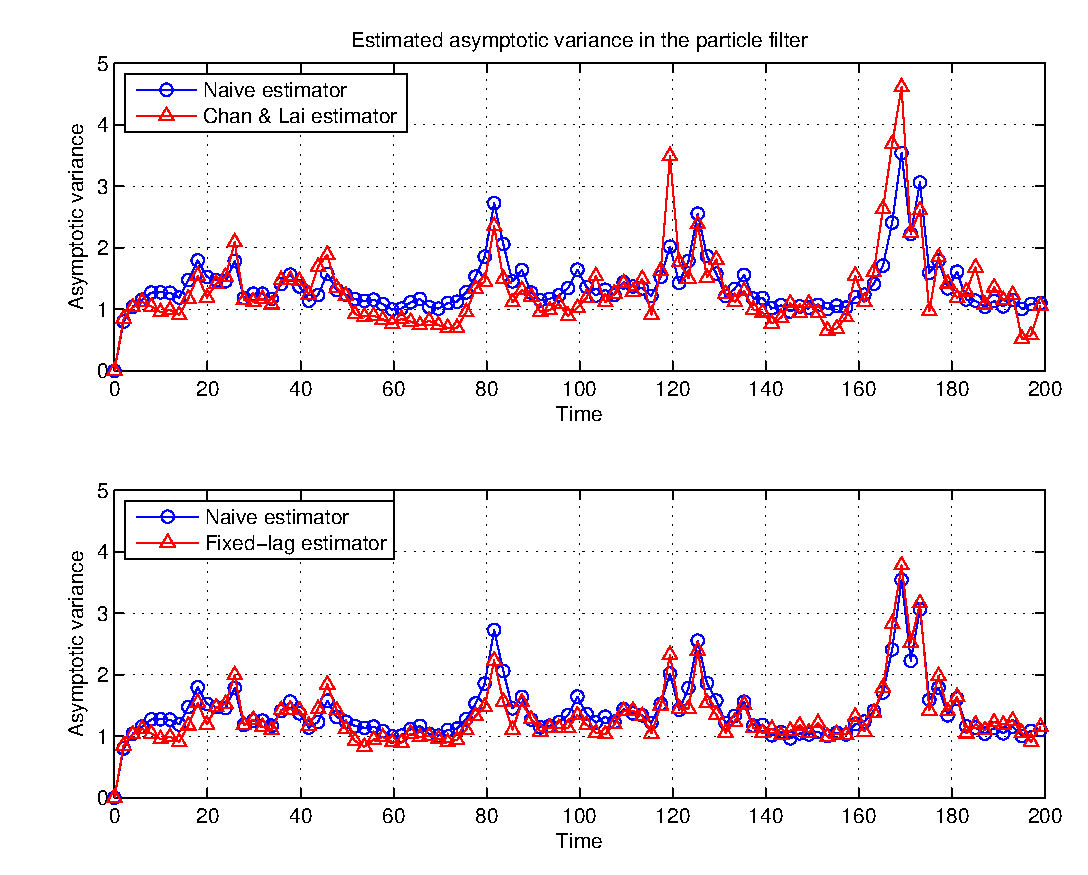
\includegraphics[width=0.8\textwidth]{variance_evolution_161214}
%\vspace{-30mm}
\caption{Long-term evolution of estimated asymptotic variances of particle predictor means in the stochastic volatility model \eqref{eq:sto:vol:model}. For clarity, only every second estimate is plotted. 
The top panel displays variance estimates ($\circ$) produced using the CLE estimator along with reference values obtained as the sample variances (scaled by the number of particles) computed from $1200$ independent replicates of the particle predictor mean sequence. The bottom panel displays the analogous plot for estimates ($\circ$) produced using the fixed-lag estimator with $\lag = 20$. The number of particles was set to $\N = 5000$ is all cases.}
 \label{fig:variance:evolution:short}
\end{figure}

\begin{figure}[H] % data in variance_evolution_161214b.mat
%\vspace{-25mm}
\centering
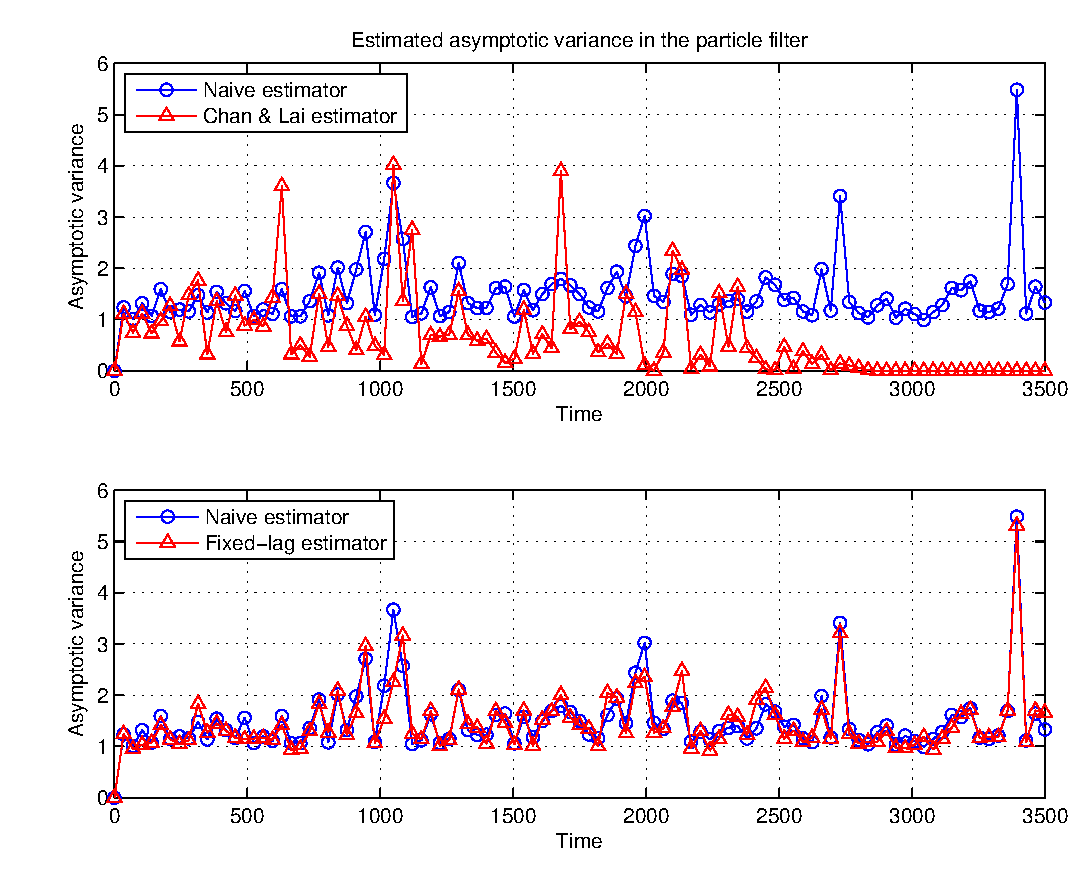
\includegraphics[width=0.8\textwidth]{variance_evolution_161214b}
%\vspace{-30mm}
\caption{The same plot as in Figure~\ref{fig:variance:evolution:short}, but now for the full observation record comprising $3500$ observations. For clarity, only every $35^{\mathrm{th}}$ estimate is plotted.}
\label{fig:variance:evolution:long}
\end{figure}



\subsection{SMC confidence bounds}
\label{sec:lin:Gauss:model}

The \emph{linear Gaussian state-space model}
\begin{equation} \label{eq:lin:Gauss:model}
\begin{split}
X_{n + 1} &= \varphi X_n + \sigma_u U_{n + 1}, \\
Y_n &= X_n + \sigma_v V_n,   
\end{split}
\quad n \in \nset, 
\end{equation}
where $\{ U_n \}_{n \in \nsetpos}$ and $\{ V_n \}_{n \in \nset}$ are again sequences of uncorrelated standard Gaussian noise, allows predictor means to be computed in a closed form using \emph{Kalman prediction} (see, e.g., \cite[Algorithm~5.2.9]{cappe:moulines:ryden:2005}). Thus, allowing comparisons with true quantities to be made, the class of linear Gaussian models is often used as a testing lab for SMC algorithms. In the setting where $|\varphi| < 1$, the state and observation processes are stationary, with zero mean Gaussian marginal stationary distributions with variances $\tilde{\sigma}^2$ and $\tilde{\sigma}^2 + \sigma_v^2$, respectively, where $\tilde{\sigma}^2 \eqdef \sigma_u^2 / (1 - \varphi^2)$. We let the former initialise the state process. 

Arguing along the lines of Section~\ref{sec:stochastic:volatility}, Assumptions~\A[assum:likelihoodDrift]{assum:majo-g} are checked straightforwardly also for this model. We leave the details to the reader.   

After having generated, for the parameterisation $(\varphi, \sigma_u, \sigma_v) = (.98, .2, 1)$, an observation record of $600$ observations, the experiment in Section~\ref{sec:lag:size:influence} was repeated for the same set of lag sizes $\lag$. As in the stochastic volatility example, the evolution of the $\N = 4000$ particles followed the same model dynamics as that generating the observations, and the reference value $1.102$ of the variance at $n = 600$ was obtained on the basis of $1000$ predictor mean replicates. The outcome is reported in Figure~\ref{fig:boxplots:lin:Gauss} and Table~\ref{tab:lags:means:stds:lin:Gauss}, which for this model indicate a somewhat even more robust performance of our estimator with respect to the lag size; indeed, more or less all the lag sizes in the interval $\intvect{12}{22}$ yield negligible biases, with only a slight increase of variance for the larger ones. According to Table~\ref{tab:lags:means:stds:lin:Gauss}, $\lambda = 18$ yields the minimal bias. As in the previous example, The CLE (corresponding to the lag size $\lambda = 600$) exhibits very unstable performance due to the relatively high $n$-to-$\N$ ratio, with at least $75\%$ of its estimates falling below the reference value. 

\begin{figure}[H] 
%\vspace{-25mm}
\centering
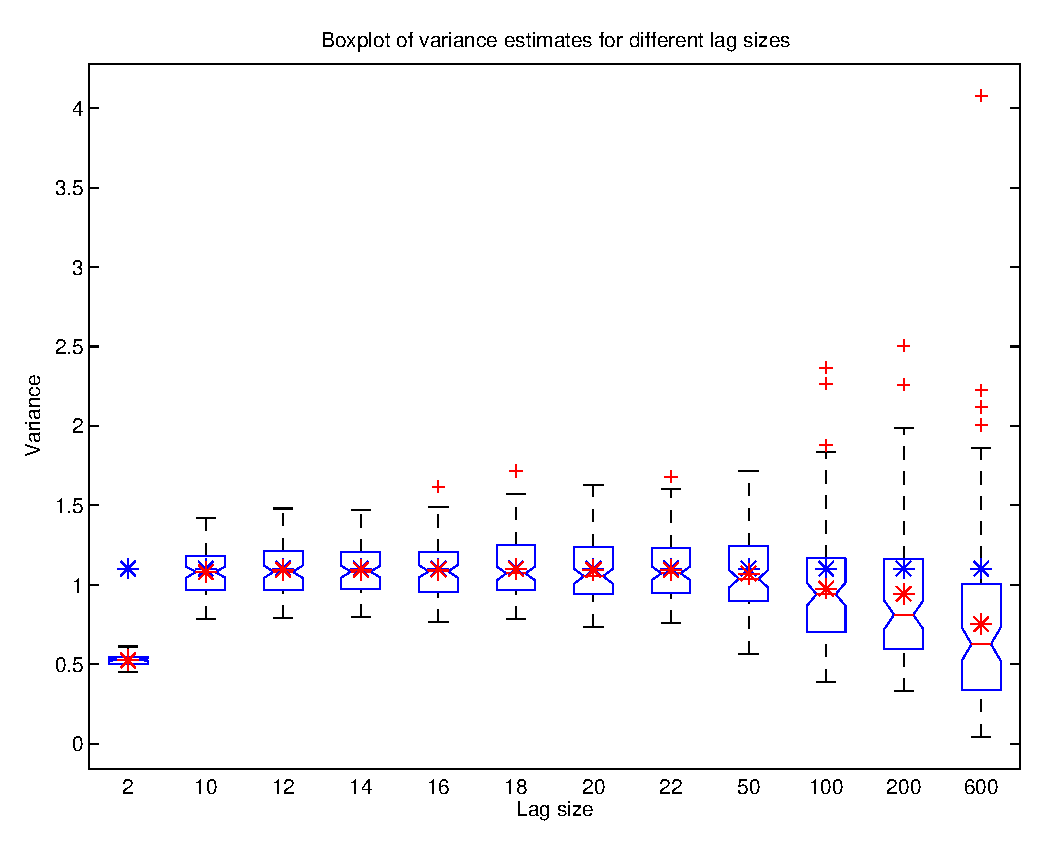
\includegraphics[width=0.8\textwidth]{boxplots_lin_Gauss_161220} % Data in fixed_lag_stovol_161220.mat
%\vspace{-30mm}
\caption{Estimated asymptotic variances of the particle predictor mean at time $600$ in the linear Gaussian model \eqref{eq:lin:Gauss:model}. The particle population size is $\N = 4000$. The boxes are based on $100$ replicates of Algorithm~\ref{alg:fixed-lag:SMC} and correspond to the different lags $\lag \in \{2, 10, 12, 14, 16, 18, 20, 22, 50, 100, 200, 600\}$. The reference value $1.102$, which is indicated by blue-colored asterisks $(\ast)$, was obtained as the sample variance (scaled by the number of particles) of $1000$ independent replicates of the particle predictor mean at time $600$ (again, Algorithm~\ref{alg:fixed-lag:SMC} used $\N = 4000$ particles). Red-colored asterisks indicate average estimates of the boxes.}
\label{fig:boxplots:lin:Gauss}
\end{figure}

\begin{table}[H] 
\begin{center}
\begin{tabular}{c|c|c} \toprule
    $\lambda$ & Mean & St. dev. \\ \midrule 
    $2$     & $.524$   & $.035$ \\
    $10$   & $1.080$ & $.157$ \\ 
    $12$   & $1.095$ & $.163$ \\
    $14$   & $1.095$& $.162$ \\
    $16$   & $1.096$ & $.175$ \\
    $18$   & $1.099$ & $.190$ \\
    $20$   & $1.094$ & $.198$ \\
    $22$   & $1.093$ & $.202$ \\
    $50$   & $1.071$ & $.246$ \\
    $100$ & $.976$   & $.370$ \\
    $200$ & $.944$   & $.471$ \\
    $600$ & $.751$   & $.593$ \\
\bottomrule
%
\end{tabular} 
\end{center}
\caption{Means and standard deviations of the variance estimates reported in Figure~\ref{fig:boxplots:lin:Gauss}. The reference value is $1.102$} 
\label{tab:lags:means:stds:lin:Gauss}
\end{table}

Finally, using the lag $\lag = 18$ extracted from the previous simulation, Algorithm~\ref{alg:fixed-lag:SMC} was re-run $150$ times on the same observation record $\chunk{y}{0}{n - 1}$, $n = 600$, each run producing a sequence $\{ \predpart[\chunk{y}{0}{m - 1}](\operatorname{id}) \}_{m = 0}^n$ of particle predictor means, a sequence $\{ \varest{\chunk{y}{0}{m - 1}}[\lagtime{m}{\lag}](\operatorname{id}) \}_{m = 0}^n$ of fixed-lag variance estimates, and associated approximate $95\%$ confidence intervals $\{ I_m \}_{m = 0}^n$, each interval given by    
\begin{equation} \label{eq:confidence:bound}
I_m = \left(\predpart[\chunk{y}{0}{m - 1}] \operatorname{id} \pm \lambda_{.025} \frac{\varest{\chunk{y}{0}{m - 1}}[\lagtime{m}{\lag}](\operatorname{id})}{\sqrt{\N}} \right), 
\end{equation}
where $\lambda_{.025}$ denotes the $2.5\%$ quantile of the standard Gaussian distribution. As before, $\N$ was set to $4000$. In the case of effective variance estimation, one may expect each $I_m$ to fail to cover the true predicted mean $\pred[\chunk{y}{0}{m - 1}](\operatorname{id})$ with a probability close to $5\%$. Since we are in the setting of a linear Gaussian model, the exact predictor means $\{ \pred[\chunk{y}{0}{m - 1}](\operatorname{id}) \}_{m = 0}^n$ are accessible through Kalman prediction, and we are thus able to assess the failure rates of the confidence intervals at different time points. Such failure rates are reported in Figure~\ref{fig:stemplot:FRs}, and the red-dashed line indicates the perfect rate $5\%$. For readability, only every $10^{\mathrm{th}}$ time point is reported. Appealingly, it is clear that the rates fluctuate constantly around $5\%$, without any notable time dependence. This re-confirms the numeric stability of our fixed-lag variance estimator. The average failure rate across all $600$ time points was $5.5\%$. The fact that the average failure rate is slightly above the perfect rate $5\%$ is in line with the fact that the bias of our estimator is always positive, as underestimation of variance leads to more narrow confidence bounds and, consequently, higher failure rates. One way of hedging against underestimation of variance could be to replace Gaussian quantiles by the quantiles of some Student's $t$-distribution with a moderate number of degrees of freedom.  

\begin{figure}[H] 
%\vspace{-25mm}
\centering
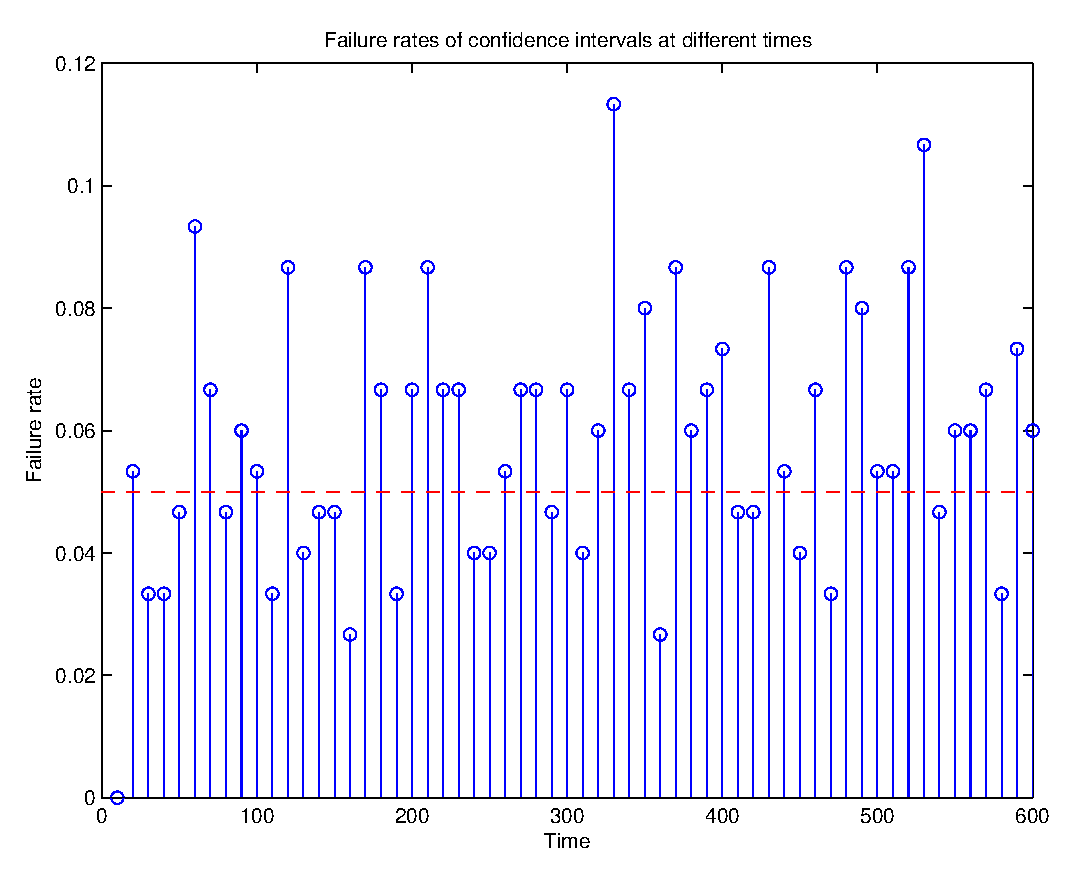
\includegraphics[width=0.8\textwidth]{stemplot_FRs} % Data in fixed_lag_lin_Gauss_161220.mat
%\vspace{-30mm}
\caption{Failure rates of confidence bounds \eqref{eq:confidence:bound} at time points $m \in \{10, 20, 30, \ldots, 600\}$. The red-dashed line indicates the perfect rate $5\%$. The failure rate estimates are based on $150$ runs of Algorithm~\ref{alg:fixed-lag:SMC} with $\N = 4000$ particles.}
\label{fig:stemplot:FRs}
\end{figure}



